%%% Frontiers in Artificial Intelligence — Original Research
%%% "Disclosed Intelligence: A Large-Sample Measurement of AI Disclosure in U.S. Investment Adviser Fiduciary Filings"
%%% Compile: pdflatex -> bibtex -> pdflatex -> pdflatex

\documentclass[utf8]{FrontiersinHarvard} % Harvard (author-date) style used by Frontiers in Artificial Intelligence

\usepackage{url,hyperref,lineno,microtype,subcaption}
\usepackage{booktabs}
\usepackage[onehalfspacing]{setspace}

\linenumbers

\def\keyFont{\fontsize{8}{11}\helveticabold }
\def\firstAuthorLast{Chincholikar {et~al.}}
\def\Authors{Samir Chincholikar\,$^{1}$ and Robin Chawla\,$^{1,*}$}
\def\Address{$^{1}$Independent Researcher}
\def\corrAuthor{Robin Chawla}
\def\corrEmail{robin.chawla.cse14@iitbhu.ac.in}

\begin{document}
\onecolumn
\firstpage{1}

\title[Disclosed Intelligence]{Disclosed Intelligence: A Large-Sample Measurement of AI Disclosure in U.S. Investment Adviser Fiduciary Filings}

\author[\firstAuthorLast ]{\Authors}
\address{}
\correspondance{}
\extraAuth{}

\maketitle

\begin{abstract}
\section{}
Industry surveys report that a majority of registered investment advisers (RIAs) now use artificial intelligence (AI), but what advisers commit to in their legally binding fiduciary disclosures is largely unmeasured. We provide the first large-sample, classifier-based measurement of AI disclosure in U.S. Form ADV Part 2A brochures. From the SEC Form ADV Part 1 structured data (16{,}223 active SEC-registered advisers reporting regulatory AUM), we draw a stratified random sample of 400 firms (adviser type $\times$ assets-under-management quartile) and retrieve each firm's current brochure from the Investment Adviser Public Disclosure system; brochures were classified for 388 firms (the remaining 12, all in the wealth/retail strata, were brochure-exempt or yielded no usable text). A five-label typology---AI in the investment process, in operations/client service, as a disclosed risk factor, explicit non-use, and named vendor---is applied by a large language model, checked for same-family reproducibility and validated by an independent, blinded re-coding of 180 brochures by a different model family, with metrics design-weighted to the population (any-use $\kappa = 0.74$, recall 0.84, precision 0.76). We report three results with design-based confidence intervals. First, disclosed AI use is low and steeply stratified: 23.7\% of brochures (95\% CI 19.7--28.2) disclose any use, increasing strongly with adviser size from about 9\% among small advisers to 30\% (wealth/retail) and 56\% (private-fund) among the largest, with strong trend and adviser-type effects (logistic regression, both $p < 0.001$). A survey-weighted estimate that reweights the strata to the brochure-filing population is 22.7\% (95\% CI 18.7--26.6), close to the design estimate, so disclosed use is robust to the sampling design. Second, the most common disclosure mode is a risk warning (27.6\%), not a claim of use. Third, potential AI-washing exposure---language resembling conduct the SEC has charged---is rare in brochures (five documents, 1.3\%; on adjudication none is an unsubstantiated promotional claim of the charged type) and, in a matched 283-firm comparison, no larger in current marketing; firms disclose AI use more in the lawyered brochure (23.0\%) than on their websites (5.7\%). We frame the survey-versus-disclosure comparison as a benchmark divergence between differently defined measures, not a validated nondisclosure rate, and we detail reliability, weighting, and scope limitations.

\tiny
 \keyFont{ \section{Keywords:} artificial intelligence, generative AI, investment advisers, Form ADV, fiduciary disclosure, text classification, large language models, AI-washing}
\end{abstract}

\section{Introduction}

Generative artificial intelligence has moved from research demonstration to a claimed business capability across financial services within a few years. Industry surveys report that a majority of registered investment advisers (RIAs) use or are piloting AI, and the Charles Schwab 2026 RIA and AI research study places adoption at roughly 63\% of surveyed firms. Adoption surveys capture what advisers report to pollsters; they do not capture what advisers commit to in the documents that carry legal weight---the Form ADV Part 2A ``brochure'' that every SEC-registered adviser must deliver to clients and that anchors the adviser's fiduciary and anti-fraud obligations under the Investment Advisers Act \citep{usSEC2019}. Whether, how, and where advisers disclose AI in these filings has not been measured at industry scale.

This matters because disclosure is the mechanism through which the fiduciary standard is operationalized, because the SEC brought its first two ``AI-washing'' enforcement actions in March 2024 (against Delphia and Global Predictions) for misrepresenting AI capabilities, and because a reliable, reproducible instrument for AI claims in regulatory text is a public good for a 16{,}000-firm population no team can read by hand. The concern is a close cousin of ``greenwashing,'' where firms overstate environmental credentials in ways that outrun substantiation \citep{delmas2011,lyon2015}; ``AI-washing'' raises the same gap between claimed and substantiated capability, but in a setting---fiduciary disclosure---where the claim is legally binding. Our aims are deliberately measurement-first: to build and validate such an instrument, to describe the level and distribution of disclosed AI use, and to compare disclosed use against the surveyed-use benchmark and against firms' own marketing.

\textbf{Research questions.} We ask three substantive questions and pursue one methodological aim throughout. RQ1 (level and distribution): how prevalent is disclosed AI use in adviser brochures, and how does it vary with adviser size and type? RQ2 (mode of disclosure): when advisers mention AI, do they predominantly claim to use it or warn about it as a risk? RQ3 (venue and exposure): how does disclosed use compare between the lawyered brochure and firms' own marketing, and how common is language resembling charged AI-washing conduct in each venue? Because credible answers require a trustworthy instrument, a methodological aim runs across all three: to validate large language models as a measurement tool for regulatory text by benchmarking a primary classifier against an independent, blinded, cross-family re-coding.

We draw a stratified random sample of 400 advisers from the SEC Form ADV Part 1 structured data, stratifying on adviser type (private-fund versus wealth/retail) and AUM quartile; retrieve each firm's current brochure; classify every brochure with a prespecified five-label typology using a large language model; and quantify uncertainty and reliability. Three findings emerge, each reported with design-based confidence intervals. Disclosed any-use is 23.7\% (95\% CI 19.7--28.2), increases strongly with size, and is higher for private-fund advisers at every size (trend and type effects both $p < 0.001$). The most common disclosure mode is risk-framing (27.6\%), not a claim of use. Potential AI-washing exposure is rare in brochures (1.3\%) and, in a matched comparison, no larger in current marketing; the fiduciary brochure is, if anything, the more AI-forward venue.

\textbf{On the survey-versus-disclosure comparison.} We report a divergence of about 39 percentage points between disclosed any-use (23.7\%) and the 63\% surveyed-use benchmark. We are explicit that this is a benchmark divergence between two differently defined measures---different populations (all SEC registrants versus Schwab-custodied survey respondents), different dates, adviser-level versus firm-level reporting, and experimental or administrative ``use'' versus material, disclosable use---and not a validated within-firm nondisclosure rate. It is informative as a contextual benchmark divergence, but the point estimate should not be read as the fraction of AI adopters who fail to disclose---the survey could overstate organizational adoption, and brochures could capture algorithmic practices respondents would not call ``AI.'' Establishing that quantity would require matched adoption information for the sampled firms, which we flag as the natural next step.

Our contributions are fourfold. First, we build a prespecified, reproducible five-label typology for AI claims in adviser filings---fixed and frozen before any outcome was examined---and validate it, reporting same-family reproducibility and, more demanding, an independent cross-family re-coding, so the paper doubles as a case study in validating LLM annotation of high-stakes regulatory text against an independent reference, an increasingly needed practice as language models are adopted as measurement instruments \citep{gilardi2023,tornberg2023,ziems2024,rathje2024,ollion2024}. Second, we provide the first large-sample estimate of disclosed AI use and its size and adviser-type gradient, with design-based inference and survey weighting to the population. Third, we distill an enforcement-anchored exposure screen from the two SEC AI-washing orders and adjudicate every positive. Fourth, we compare disclosure across the fiduciary brochure and firms' own marketing, and release a complete reproducibility artifact. The whole design extends the tradition of using filing text as a firm-level measurement instrument \citep{tetlock2007,loughran2011,hoberg2016,cohenLazy2020,abis2022} to a new and policy-salient attribute. Section 2 situates the study; Section 3 gives data, methods, and inference; Section 4 reports results, including robustness; Section 5 discusses mechanisms, regulation, and limitations.

\section{Institutional Background and Related Literature}

\subsection{Form ADV and the fiduciary brochure}
Every SEC-registered adviser files Form ADV. Part 1 is structured, machine-readable firm data (legal name, CRD identifier, regulatory AUM, client counts, private-fund activity, disciplinary history), published by the SEC as bulk data. Part 2A, the brochure, is a narrative plain-English document describing the adviser's business, strategies, fees, conflicts, and material risks; it must be delivered to clients and is the primary written expression of the adviser's disclosure obligations. Because the brochure describes how an adviser actually manages money, it is where disclosed AI use should appear, and where misstatements about AI carry the clearest legal consequence.

\subsection{AI-washing enforcement}
On 18 March 2024 the SEC settled charges against two advisers for false or misleading AI statements. Delphia (USA) Inc. claimed it used ``machine learning to analyze the collective data'' in a ``predictive algorithmic model'' it had not developed (US \$225{,}000 penalty); Global Predictions Inc. billed itself the ``first regulated AI financial advisor'' with ``[e]xpert AI-driven forecasts'' it could not substantiate (US \$175{,}000) \citep{usSEC2024a,usSEC2024b}. These orders establish that promotional AI claims are actionable and provide a textual fingerprint of charged conduct against which live disclosures can be screened.

\subsection{Related literature}
\textbf{Text as a firm-level measurement instrument.} A large literature treats corporate and regulatory text as data from which a firm attribute can be measured. \citet{loughran2011,loughran2016} show that domain-specific dictionaries are required to read financial disclosure, because general sentiment lexicons mislabel routine legal language; \citet{tetlock2007} links media text to market outcomes; \citet{hoberg2016} build product-market classifications from 10-K text; and \citet{cohenLazy2020} show that changes in filing language are economically informative. \citet{abis2022} is our closest design template: she classifies mutual-fund prospectus text to separate quantitative from discretionary managers and links the classification to fund behavior. \citet{gentzkow2019} survey the econometrics of text as data, and \citet{grimmer2013} codify the validation discipline---no measurement from text is credible without an explicit reliability check against an independent standard---which we take seriously here. We adapt this tradition to a new attribute: disclosed use of AI in the document that carries an adviser's fiduciary obligations.

\textbf{Large language models as annotators.} A fast-moving methodological literature asks whether LLMs can replace or augment human coders for text annotation. \citet{gilardi2023} find ChatGPT outperforms crowd workers on several annotation tasks; \citet{tornberg2023} reports strong zero-shot performance on political text; \citet{ziems2024} map where LLMs can and cannot substitute for human labor in computational social science; and \citet{rathje2024} validate LLM-based measurement across languages. A cautionary strand warns that proprietary, versioned models threaten reproducibility and can embed systematic error that agreement statistics alone will not reveal \citep{ollion2024,bommasani2021}. We treat these cautions as design constraints: we freeze a model snapshot and rubric, report same-family reproducibility, and---critically---benchmark the primary classifier against an independent re-coding from a different model family, distinguishing reproducibility from accuracy throughout.

\textbf{Economics of AI adoption, disclosure, and ``washing.''} The economics of AI adoption motivate why disclosure is worth measuring: AI reshapes labor demand \citep{acemoglu2022}, firm growth and innovation \citep{babina2024}, firm value \citep{eisfeldt2023}, and worker productivity \citep{noy2023,brynjolfsson2025}, and prediction technologies are reorganizing financial services specifically \citep{agrawal2018,dacunto2019}. \citet{babina2024} measure adoption from job postings; the divergence between adoption so measured and fiduciary disclosure is our object of study. Disclosure theory frames why firms may reveal or withhold \citep{verrecchia2001,healy2001,leuz2016,blankespoor2020}, and a recent strand studies strategic disclosure when machines read filings \citep{cao2024}. Finally, the phenomenon we screen for is the AI analogue of greenwashing, where claimed credentials outrun substantiation \citep{delmas2011,lyon2015}. To our knowledge this is the first large-sample, classifier-based, independently validated measurement of AI disclosure in adviser fiduciary filings.

\section{Data and Methods}

\subsection{Sampling frame and stratified sample}
The frame is the SEC Form ADV Part 1 structured data (adviser base table). We keep each firm's most recent filing and restrict to firms active through 2024. From 27{,}679 unique CRD identifiers filing between 2011 and 2024, this yields 16{,}709 active registrants, of which 16{,}223 report regulatory AUM and constitute the sampling and weighting universe. We draw a stratified random sample of 400 firms with a fixed seed, crossing adviser type---private-fund (Item 7.B) versus wealth/retail---with AUM quartile (Item 5.F.(2)(c) total regulatory AUM), eight cells of 50. The sample is frozen before any brochure is read. Equal allocation deliberately over-samples large advisers relative to the small-firm-dominated population; we therefore report both design-based (unweighted) and survey-weighted estimates (Section 3.7). The Part 1 bulk data reflect filings through 31 December 2024, and adviser type and AUM quartile are therefore measured using the latest 2024 filing available in the sampling frame. Brochures, marketing pages, classification, and validation were observed in 2026. The resulting temporal difference between the 2024 stratification variables and the 2026 disclosure observations is a design limitation; the 2024 attributes are used to define the frozen sampling strata rather than interpreted as contemporaneous 2026 firm characteristics. The design targets prevalence estimation rather than fine within-cell contrasts: at $n = 388$ the overall any-use rate is estimated to a Wilson half-width of about $\pm 4$ percentage points, and roughly 50 firms per cell give within-stratum half-widths of about $\pm 9$--12 points---adequate to resolve the size and adviser-type gradient we report, but not fine differences between adjacent cells, which we do not interpret.

\subsection{Brochure retrieval and classified denominators}
For each firm we obtain the current Part 2A brochure version identifier from the IAPD firm API, retrieve the brochure PDF, and extract its text. Text was classified for 388 of 400 firms. The 12 firms without a classified brochure are all in the wealth/retail strata: 11 returned an IAPD Part-2-brochure-exempt flag and one retrieved document yielded no usable text. Because these fall in the wealth cells, wealth-stratum denominators are 46--48 rather than 50, which we carry through all per-cell estimates. The estimand is disclosure among advisers that file a Part 2A brochure; brochure-exempt firms have no brochure and are excluded from the disclosure estimand rather than counted as zero-disclosers, and the single unretrievable document is treated as missing. Because exemptions are rare (11 of 400), an alternative that counted exempt firms as non-disclosers would lower the prevalence by at most about three percentage points and would not change any conclusion. Retrieval respected the host's fair-access expectations; raw documents were persisted with content hashes.

\subsection{The claim typology}
The instrument is a five-label, multi-label typology, fixed before analysis: (a) AI in the investment process; (b) AI in operations/client service; (c) AI as a disclosed risk factor; (d) explicit prohibition/non-use; (e) a named AI vendor/product invoked as an AI capability. Derived indicators are any-use (a $\cup$ b $\cup$ e) and any-mention (a $\cup$ b $\cup$ c $\cup$ d $\cup$ e). Because label (e) records only that a vendor is named---not necessarily that the adviser materially uses it---we report any-use both including and excluding (e). A label is assigned only when a verbatim passage supports it. The full rubric, prompts, keyword-window rules, model snapshot and date, and decision rules are deposited (Section 6).

\subsection{LLM classification and reliability}
Classification is tooling; the object of study is the industry. AI-relevant passages are extracted by keyword windowing and submitted with the frozen rubric to a large language model (OpenAI gpt-4o, fixed snapshot, temperature 0) that returns structured labels. We assess reliability at two levels. Inter-model reproducibility: a random 60-brochure subsample is re-classified by a second model from the same family (gpt-4o-mini) and we report per-label percent agreement and Cohen's $\kappa$ \citep{cohen1960}; agreement between two same-family models establishes reproducibility, not accuracy. Independent cross-family validation: a blinded 180-brochure set is re-coded from the brochure text and the frozen rubric alone by an independent rater from a different model family (Anthropic Claude), with no access to the primary labels. The validation set is a two-phase (verification) sample, not a simple random sample: it comprises all 123 brochures the primary classifier assigned any label (a ``positive'' means any of a--e, i.e., any mention; these are taken as a census, inclusion probability 1) plus a random sample of 57 of the 265 model-negative brochures (inclusion probability $57/265 = 0.215$; seed 42). This enrichment is deliberate---it observes every potential false positive and a representative fraction of potential false negatives---but it means raw metrics computed on the 180 do not directly estimate population operating characteristics. We therefore report design-weighted (Horvitz--Thompson) precision, recall, F1, Cohen's $\kappa$, percent agreement, and prevalence-and-bias-adjusted agreement (PABAK; \citealp{byrt1993}), weighting each brochure by the inverse of its inclusion probability so the estimates apply to the full classified population; precision, being conditional on the fully censused model-positive stratum, is unaffected by the weighting, whereas recall and $\kappa$ are. Because both raters are language models, this measures cross-family, cross-instrument agreement against a common rubric---stronger than the same-family check (larger sample, fully blinded, independent family) but not a substitute for a panel of human domain experts; we therefore enumerate the full residual disagreement set so a targeted human audit can adjudicate the boundary cases (Supplementary Material S2). The coding sheet, the independent codes, and the scoring code are provided so the step is fully auditable. Total metered classification cost was under two U.S. dollars.

\subsection{The exposure screen}
From the text of the Delphia and Global Predictions orders we distill seven promotional-claim patterns (F1--F7: predictive-power, first-mover/identity, edge/alpha, AI-manages-portfolios, learns-from-data, quantified-capability, and AI-as-headline-differentiator). A document is flagged if it makes a claim materially similar to any pattern. We deliberately term this a potential exposure-language screen: it measures textual similarity to charged conduct, not misconduct; the fingerprint is distilled from only two cases; positives are few; and every positive is individually adjudicated with the passage quoted (Supplementary Material S1). All results are aggregate and no firm is identified.

\subsection{Marketing corpus, venue comparison, and missingness}
To test venue substitution, we assemble a current marketing corpus for the sampled firms. Each firm's website is resolved from its brochure; the homepage and principal descriptive pages (about, approach, technology) are crawled (one request per second per host, up to eight pages, main-text extraction) and classified with the same typology and exposure screen. Usable marketing text was obtained for 283 firms. We characterize selection explicitly (Section 4.5): we compare firms with and without usable marketing text on adviser type, AUM quartile, and regulatory AUM. The comparison is limited to current main-site pages; JavaScript-rendered content, press releases, social media, and historical campaigns are out of scope, a limitation we foreground because the enforcement claims themselves appeared in such channels.

\subsection{Inference and weighting}
We report Wilson 95\% confidence intervals for every prevalence, per label and per stratum. We test the AUM gradient with a linear-by-linear trend test within each adviser type and overall, and estimate a firm-level logistic regression of any-use on AUM quartile (ordinal) and adviser type. The venue difference is tested with a paired bootstrap. For population inference we compute a survey-weighted any-use prevalence over the estimand's population---brochure-filing advisers. Each stratum's exact population count (from applying the identical stratification to the full frame) is deflated by the stratum's observed brochure-filing rate to estimate the brochure-filing population, and each stratum's sample prevalence is weighted by its share of that universe, with a stratified design-based variance. Using the unadjusted all-AUM-reporting universe (16{,}223 firms) instead yields essentially the same value (22.3\% vs.\ 22.7\%), confirming that the small brochure exemptions do not affect the estimate. Weighted and unweighted estimates are reported side by side (Table~\ref{tab:weighting}). In brief: equal allocation across strata estimates the sample efficiently, and the survey weights recover the brochure-filing population by weighting each stratum by its population share---the stratum's exact population count from the full frame, deflated by its observed brochure-filing rate---so the weighted figure answers ``what share of brochure-filing advisers disclose,'' while the unweighted figure describes the stratified sample itself.

\section{Results}

\subsection{Typology distribution}
Table~\ref{tab:typology} and Figure~\ref{fig:typology} report each label's prevalence with Wilson 95\% CIs across the 388 classified brochures. Disclosed any-use (a $\cup$ b $\cup$ e) is 23.7\% (19.7--28.2); excluding the named-vendor label, any-use of (a $\cup$ b) is 20.9\%. Any AI mention is 31.7\% (27.3--36.5). The most common single label is AI as a disclosed risk factor (27.6\%), exceeding investment-process use (18.3\%): advisers more often warn about AI than claim to use it. Explicit non-use (d) is essentially absent.

\begin{table}[!ht]
\caption{Typology prevalence with Wilson 95\% confidence intervals (gpt-4o classifier; $n = 388$ classified brochures). Labels are multi-label.}
\label{tab:typology}
\centering
\begin{tabular}{lrr}
\toprule
Label & $k / n$ & Prevalence (95\% CI) \\
\midrule
(a) AI in investment process & 71 / 388 & 18.3\% (14.8--22.5) \\
(b) AI in operations / client service & 26 / 388 & 6.7\% (4.6--9.6) \\
(c) AI as a disclosed risk factor & 107 / 388 & 27.6\% (23.4--32.2) \\
(d) Explicit prohibition / non-use & 8 / 388 & 2.1\% (1.0--4.0) \\
(e) Named AI vendor / product & 21 / 388 & 5.4\% (3.6--8.1) \\
Any use (a $\cup$ b $\cup$ e) & 92 / 388 & 23.7\% (19.7--28.2) \\
Any mention (a--e) & 123 / 388 & 31.7\% (27.3--36.5) \\
\bottomrule
\end{tabular}
\end{table}

\subsection{Size and type gradient}
Table~\ref{tab:gradient} and Figure~\ref{fig:gradient} show disclosed any-use by stratum with denominators and CIs. Any-use rises monotonically with AUM among private-fund advisers (12\%$\rightarrow$24\%$\rightarrow$34\%$\rightarrow$56\%) and broadly increases among wealth/retail advisers (8.7\%, 8.3\%, 14.6\%, 30.4\%; the Q1--Q2 difference is within sampling error), and private-fund advisers disclose more at every quartile. A linear-by-linear trend test confirms the gradient (private fund $z = 4.82$, $p < 10^{-5}$; wealth/retail $z = 3.00$, $p = 0.003$; overall $z = 5.57$, $p < 10^{-7}$). In a firm-level logistic regression of any-use on AUM quartile (ordinal) and adviser type, both predictors are significant (AUM quartile: coefficient 0.67, SE 0.12, $p < 0.001$; private-fund: coefficient 1.01, SE 0.27, $p < 0.001$), and private-fund advisers disclose at 31.5\% versus 15.4\% for wealth/retail ($\chi^2$ $p = 0.0003$).

\begin{table}[!ht]
\caption{Disclosed any-use by adviser type and AUM quartile: prevalence (Wilson 95\% CI) [count/denominator]. Wealth/retail denominators are below 50 because the 12 unclassified firms fall in these strata.}
\label{tab:gradient}
\centering
\small
\begin{tabular}{lcccc}
\toprule
Adviser type & Q1 & Q2 & Q3 & Q4 \\
\midrule
Private fund & 12\% (6--24) [6/50] & 24\% (14--37) [12/50] & 34\% (22--48) [17/50] & 56\% (42--69) [28/50] \\
Wealth / retail & 8.7\% (3--20) [4/46] & 8.3\% (3--20) [4/48] & 14.6\% (7--27) [7/48] & 30.4\% (19--45) [14/46] \\
\bottomrule
\end{tabular}
\end{table}

\subsection{The survey-versus-disclosure divergence}
Table~\ref{tab:weighting} reports the eight-stratum brochure-filing population counts, sample sizes, disclosure rates, and sampling weights. Reweighting the strata to the brochure-filing population yields a survey-weighted any-use prevalence of 22.7\% (95\% CI 18.7--26.6), close to the design-based estimate of 23.7\% (19.7--28.2); the unadjusted all-firms universe gives 22.3\%. Wealth/retail advisers collectively account for about 64\% of the weighting universe and have a population-weighted disclosure rate well below that of private-fund advisers (their two smallest-AUM strata disclose about 8\%, though their largest discloses 30\%); the large private-fund strata disclose enough (up to 56\%) that the weighted estimate remains near the design value. Disclosed use is therefore robust to the sampling design rather than an artifact of over-sampling large firms. Against the 63\% surveyed-use benchmark the divergence is about 40 percentage points weighted and 39 unweighted. As stated in Section 1 and Section 5.1, this is a divergence between differently defined measures, not a within-firm nondisclosure rate; the near-equality of the weighted and unweighted estimates simply shows the divergence does not depend on the design.

\begin{table}[!ht]
\caption{Brochure-filing population counts (exact stratum population deflated by the stratum brochure-filing rate), classified sample sizes, disclosure rates, and sampling weights. The survey-weighted any-use prevalence is 22.7\% (95\% CI 18.7--26.6) versus the design-based 23.7\%; the unadjusted all-firms universe (16{,}223) gives 22.3\%.}
\label{tab:weighting}
\centering
\begin{tabular}{lrrrr}
\toprule
Stratum & Filing pop.\ $N$ & Class.\ $n$ & Any-use & Weight \\
\midrule
Private fund $\cdot$ Q1 & 769 & 50 & 12.0\% & 0.049 \\
Private fund $\cdot$ Q2 & 1{,}060 & 50 & 24.0\% & 0.068 \\
Private fund $\cdot$ Q3 & 1{,}604 & 50 & 34.0\% & 0.103 \\
Private fund $\cdot$ Q4 & 2{,}449 & 50 & 56.0\% & 0.157 \\
Wealth/retail $\cdot$ Q1 & 3{,}271 & 46 & 8.7\% & 0.210 \\
Wealth/retail $\cdot$ Q2 & 2{,}790 & 48 & 8.3\% & 0.179 \\
Wealth/retail $\cdot$ Q3 & 2{,}268 & 48 & 14.6\% & 0.145 \\
Wealth/retail $\cdot$ Q4 & 1{,}397 & 46 & 30.4\% & 0.090 \\
Total (weighted) & 15{,}606 & 388 & 22.7\% & 1.000 \\
\bottomrule
\end{tabular}
\end{table}

\subsection{Reliability}
Reliability is assessed at two levels. Same-family inter-model agreement on the 60-brochure subsample is near-perfect for the risk-factor label ($\kappa = 0.95$), named-vendor ($\kappa = 1.00$), and any-mention ($\kappa = 0.86$), and moderate for the finer use distinctions (investment-process $\kappa = 0.61$; operations $\kappa = 0.66$; any-use composite $\kappa = 0.69$); the prohibition label has near-zero prevalence, so its $\kappa$ is undefined. The stronger test is the independent cross-family validation of Table~\ref{tab:validation} and Figure~\ref{fig:validation}, in which all 180 blinded brochures were re-coded by a different model family with no access to the primary labels. Because the 180 are a two-phase verification sample (Section 3.4), Table~\ref{tab:validation} reports design-weighted metrics that apply to the full classified population. On these weighted estimates the reliable constructs are confirmed---risk factor $\kappa = 0.93$ (F1 = 0.95), named vendor recall 1.00---and the headline estimand is well recovered: the any-use indicator reaches $\kappa = 0.74$ with recall 0.84 and precision 0.76 (precision is unaffected by the weighting because model-positives are censused). The finer investment-process label remains the softest construct ($\kappa = 0.65$), and the full disagreement analysis (Supplementary Material S2) shows why: the classifier over-calls investment-process AI on reserve-the-right-to-use language, third-party or execution algorithms, and rule-based robo-advice, and it over-calls named-vendor when a product (e.g., ChatGPT) is named only illustratively; in the opposite direction it misses some firms' own quantitative-model investing. Combining the design-weighted precision and recall implies a validation-adjusted any-use prevalence of about 21.6\% (from the cross-family error rates, not human adjudication), inside the design-based confidence interval (19.7--28.2) and, because the correction is downward, only widening the divergence against surveyed adoption (we treat this as a sensitivity estimate in Section 4.6, not a revised headline). We accordingly designate any-use (a $\cup$ b $\cup$ e) and the risk-factor label (c) as the primary, well-validated outcomes, and report the finer investment-process label (a) as a secondary, approximate construct.

\begin{table}[!ht]
\caption{Independent cross-family validation on the blinded 180-brochure verification sample. Metrics are design-weighted (Horvitz--Thompson) to the full classified population: model-positive brochures are censused (inclusion probability 1) and 57 of 265 model-negatives are sampled (inclusion probability 0.215), so each brochure is weighted by the inverse of its inclusion probability. Reference is an independent blind re-coding by a different model family; the primary classifier is gpt-4o. Precision is invariant to the weighting (it conditions on the censused model-positive stratum); recall, $\kappa$, agreement, and PABAK are design-weighted. Same-family reproducibility (gpt-4o vs.\ gpt-4o-mini, 60 brochures) is reported in the text.}
\label{tab:validation}
\centering
\small
\begin{tabular}{lrrrrrr}
\toprule
Label / indicator & Prec. & Rec. & F1 & \% agree & $\kappa$ & PABAK \\
\midrule
(a) investment process & 0.690 & 0.735 & 0.712 & 89.8\% & 0.650 & 0.796 \\
(b) operations & 0.808 & 0.677 & 0.737 & 96.1\% & 0.716 & 0.923 \\
(c) risk factor & 0.916 & 0.990 & 0.951 & 97.4\% & 0.934 & 0.948 \\
(d) explicit non-use & 0.875 & 0.467 & 0.609 & 97.7\% & 0.598 & 0.954 \\
(e) named vendor & 0.524 & 1.000 & 0.688 & 97.4\% & 0.675 & 0.948 \\
Any use (a $\cup$ b $\cup$ e) & 0.761 & 0.837 & 0.797 & 90.8\% & 0.738 & 0.816 \\
\bottomrule
\end{tabular}
\end{table}

\subsection{Exposure and the venue comparison}
Applying the F1--F7 screen to the brochures, potential exposure language is rare: 5 of 388 brochures (1.3\%, 95\% CI 0.6--3.0). Given so few positives, each was adjudicated against the charged-conduct standard with the passage quoted (Supplementary Material S1). Two are false positives---a systematic strategy's trading mechanism and an automated managed-account program described factually---and three are substantiated, risk-disclosed descriptions of genuinely operated AI/ML investment methods (the firms name platforms or data vendors and disclose model and predictive-analysis risk). None is an unsubstantiated promotional claim of the type charged in Delphia or Global Predictions; adjudicated charged-conduct-type exposure is therefore 0 of 388 (at most one borderline but substantiated predictive-performance claim). The raw screen rate overstates exposure because the lexical pattern also matches factual quantitative, robo, and machine-learning disclosure---illustrating why the screen is reported as a prefilter requiring adjudication, not a misconduct measure.

For the 283 firms with both a classified brochure and usable marketing text, Table~\ref{tab:venue} and Figure~\ref{fig:venue} report the venue comparison. Marketing exposure equals brochure exposure in this matched set (0.7\% each; paired difference 0.000, bootstrap 95\% CI $-0.014$ to $+0.014$). Disclosed any-use is markedly higher in the brochure (23.0\%) than in marketing (5.7\%): 58 firms disclose AI use in the brochure but not on their website, versus 9 in the reverse direction. Contrary to the intuition motivating AI-washing concern, the fiduciary brochure is the more AI-forward venue. A missingness analysis limits selection concern: firms with and without usable marketing text do not differ significantly in adviser type ($\chi^2$ $p = 0.83$), AUM quartile ($\chi^2$ $p = 0.50$), or regulatory AUM (median US \$419M vs.\ US \$357M; Mann--Whitney $p = 0.46$). We nonetheless restrict this finding to the matched sample and to current main-site pages.

\begin{table}[!ht]
\caption{Venue comparison for firms with both venues ($n = 283$). The difference column is Marketing minus Brochure; the bracketed figures are a paired bootstrap 95\% CI.}
\label{tab:venue}
\centering
\begin{tabular}{lrrr}
\toprule
Measure ($n = 283$) & Brochure & Marketing & Marketing $-$ Brochure \\
\midrule
Exposure-language screen (F1--F7) & 0.7\% & 0.7\% & 0.000 ($-0.014$, $+0.014$) \\
Any-use disclosure (a $\cup$ b $\cup$ e) & 23.0\% & 5.7\% & $-17.3$ pp \\
\bottomrule
\end{tabular}
\end{table}

Table~\ref{tab:missingness} makes the marketing-corpus coverage auditable across the variables tested. Usable text is obtained for a similar share of firms in each adviser type and AUM quartile, and the median regulatory AUM of covered and uncovered firms is close; the selection tests reported above (all non-significant) can therefore be read directly against the coverage pattern.

\begin{table}[!ht]
\caption{Marketing-corpus coverage (firms with usable website text) by adviser type and AUM quartile, with median regulatory AUM of covered versus uncovered firms. Differences are non-significant (type $\chi^2$ $p = 0.83$; quartile $\chi^2$ $p = 0.50$; AUM Mann--Whitney $p = 0.46$).}
\label{tab:missingness}
\centering
\begin{tabular}{lrr}
\toprule
Group & Usable / total & Coverage \\
\midrule
Private-fund advisers & 140 / 200 & 70.0\% \\
Wealth/retail advisers & 143 / 200 & 71.5\% \\
AUM quartile Q1 (smallest) & 73 / 100 & 73.0\% \\
AUM quartile Q2 & 65 / 100 & 65.0\% \\
AUM quartile Q3 & 71 / 100 & 71.0\% \\
AUM quartile Q4 (largest) & 74 / 100 & 74.0\% \\
Median regulatory AUM & \multicolumn{2}{r}{covered US \$419M \; vs.\ \; uncovered US \$357M} \\
\bottomrule
\end{tabular}
\end{table}

\subsection{Robustness and sensitivity}
The headline results survive the natural sensitivity checks. First, definition of the estimand: dropping the named-vendor label, any-use of (a $\cup$ b) is 20.9\% versus 23.7\% for (a $\cup$ b $\cup$ e), so the level is not driven by mere vendor mentions; because named-vendor is the lowest-precision label (Section 4.4), we report it separately and treat the (a $\cup$ b) figure as a conservative floor. Second, validation-based bias correction: combining the design-weighted precision (0.76) and recall (0.84) from Section 4.4 implies a validation-adjusted any-use prevalence of about 21.6\% (adjusted using the cross-family classifier error, not human adjudication), still inside the 95\% CI (19.7--28.2) and, because the correction is downward, only widening the divergence against surveyed adoption. Because this correction relies on the two-phase validation sample, we treat it as a sensitivity estimate rather than a revised headline. Third, the unclassified firms: the 12 brochures we could not classify are all in the wealth/retail strata (brochure-exempt or without usable text); since those strata have the lowest disclosure rates, treating them as non-disclosers rather than as missing would lower the estimate by less than a percentage point and cannot generate the observed gradient. Fourth, the sampling design: the design-based (23.7\%) and survey-weighted (22.7\%) estimates agree to within a point, and the all-firms-universe weighting (22.3\%) is lower still, so the level is not an artifact of over-sampling large advisers. Fifth, reliability across instruments: the same-family (gpt-4o vs.\ gpt-4o-mini) and independent cross-family checks agree on which constructs are reliable (risk-factor, named-vendor, any-mention) and which are soft (the fine investment-process distinction), so the reliability ordering is not specific to one model pair. Sixth, the exposure screen: because it is a lexical prefilter that also matches factual quantitative, robo, and machine-learning disclosure, we adjudicate every positive by hand and report the adjudicated count (0 of 388 of the charged type) rather than the raw screen rate. Seventh, source of labels: re-estimating disclosure from the independent cross-family coder's labels over the validation sample (design-weighted) yields a population any-use prevalence of 21.6\%, close to the model-based 23.7\%, and preserves the adviser-type ordering (private-fund 24.6\% versus wealth/retail 17.6\%); the substantive pattern therefore does not depend on which model produced the labels. We did not tune the rubric, keyword window, or model after inspecting outcomes; the instrument was frozen before analysis.

\section{Discussion}

\subsection{What the divergence is, and is not}
The survey-versus-disclosure divergence combines several distinct differences: firm populations (all SEC registrants versus Schwab-custodied respondents), observation dates, adviser-level versus firm-level reporting, experimental or individual use versus material organizational use, and general technology use versus a disclosure obligation. It is therefore an informative benchmark divergence, not a validated adoption--disclosure gap, and we do not claim a single nondisclosure percentage. The paper's primary contributions are the measured level and distribution of disclosure and the instrument that produces them; the divergence is context. A design that obtained matched adoption for the sampled firms---by survey linkage or by coding adoption signals directly---would convert the divergence into a within-firm gap and is the natural extension.

\subsection{Interpreting the level and gradient}
Disclosed use is low and steeply size-graded. We observe what firms describe, not what they do: larger private-fund advisers are substantially more likely to describe AI-related investment methods in their brochures, and the long tail of small advisers describes none. The monotone size gradient is consistent with classic diffusion-of-innovation dynamics, in which larger, better-resourced organizations adopt and communicate a new technology earlier than smaller peers \citep{rogers2003}. That the dominant mode is risk-framing rather than a claim of use is consistent with two non-exclusive interpretations---post-enforcement caution and materiality judgments (many productivity or back-office uses may be immaterial to a client's investment decision and hence not brochure items)---but the cross-sectional design cannot establish that enforcement caused the caution; that would require longitudinal evidence. The significant type effect---private-fund advisers describe AI more at every size---fits their more technical brochures and audiences.

The dominance of risk-framing over use-claims deserves emphasis because it inverts the intuition behind AI-washing concern. Standard disclosure theory predicts that firms reveal favorable, verifiable information and withhold what is costly or hard to substantiate \citep{verrecchia2001,healy2001}; a promotional AI claim in a fiduciary brochure is precisely the kind of statement that is cheap to make but expensive to defend if examined, and the March 2024 orders made that expense concrete. The observed pattern---advisers warn about AI as a risk more than twice as often as they claim to use it---is what one would expect when the marginal legal cost of an unsubstantiated capability claim is high and the cost of a boilerplate risk factor is low. This is a hypothesis the cross-section is consistent with but cannot prove; a pre/post-enforcement panel would identify it. It also implies that the brochure is a conservative venue for measuring AI use: our estimates are more likely to understate than to overstate genuine adoption, reinforcing that the gap against surveyed use is not an artifact of over-counting.

\subsection{Why the lawyered document is the louder venue}
The brochure discloses AI use more often than firms' own marketing. The two genres differ: the brochure exhaustively itemizes methods, including algorithmic and quantitative ones and their risks, whereas marketing homepages are short and benefit-oriented; and post-enforcement incentives plausibly cut against promotional AI claims in every public venue (an interpretation the cross-sectional design cannot establish causally). The implication for AI-washing policy is that, in current main-site marketing, the feared venue substitution is not evident---exposure language is rare everywhere we look.

\subsection{Regulatory implications}
The reliable constructs (any-mention, risk-factor, named-vendor) can be computed across the full population to triage examinations, and the size gradient predicts where investment-process AI concentrates. The exposure screen is a low-base-rate filter for language resembling charged conduct; because such language is rare in brochures, a full deployment should also cover marketing, press, and social text and historical snapshots. Nothing here identifies misconduct: the screen measures textual similarity, not a legal conclusion, and only aggregates are reported.

\subsection{Limitations}
First, construct and comparability: the survey benchmark and the disclosure measure are not equivalent (Section 5.1). Second, scope: this is a cross-section of current brochures, not a panel; a short forward panel is the natural extension for diffusion. Third, reliability: same-family inter-model agreement establishes reproducibility, not accuracy, and the independent cross-family validation (Section 4.4, Supplementary Material S2) is itself between two language models rather than against a panel of human experts, so it bounds cross-instrument error but does not certify human-level accuracy; the fine investment-process label is therefore reported as approximate (design-weighted $\kappa = 0.65$), while the primary any-use construct shows substantial agreement ($\kappa = 0.74$) and the risk-factor construct shows almost-perfect agreement ($\kappa = 0.93$), and the enumerated disagreement set is provided for a targeted human audit. Fourth, weighting: the design over-samples large firms, but the design-based (23.7\%) and survey-weighted (22.7\%) estimates are close, so the reported level is not an artifact of the allocation. Fifth, the exposure screen rests on two enforcement cases and few positives; it is a potential-exposure-language screen with adjudicated positives, not a misconduct measure. Sixth, the venue comparison covers current main-site marketing for 283 of 400 firms; although missingness is not significantly related to size or type, JavaScript-rendered, press, social, and historical content are unobserved. Seventh, generalizability: the study covers SEC-registered investment advisers filing a Form ADV brochure in the United States, and the surveyed-use benchmark is a single industry source; the instrument transfers to other filings and jurisdictions in principle, but the specific levels reported here should not be extrapolated beyond this population.

\subsection{Future research}
Four extensions follow directly. First, a short forward panel of brochures spanning the March 2024 enforcement date would convert the cross-sectional gradient and the risk-framing pattern into causal, diffusion-style evidence and identify whether disclosure responds to enforcement. Second, obtaining matched adoption information for the sampled firms---through survey linkage or by coding adoption signals such as job postings and infrastructure directly \citep{babina2024}---would turn the benchmark divergence into a validated within-firm adoption--disclosure gap. Third, a targeted human expert audit of the enumerated disagreement set (Supplementary Material S2) would upgrade the fine investment-process label from an LLM-validated to a human-validated construct and calibrate the residual instrument error. Fourth, the frozen instrument can be applied at population scale (all $\sim$16{,}000 advisers) and extended to additional venues (press releases, Form CRS, social media) and to other regulatory-text settings, providing a reusable, auditable tool for supervisory triage. Because the complete pipeline, rubric, and data are released, each of these extensions can build directly on the artifact rather than reconstructing the instrument.

\section{Conclusion}
We provide the first large-sample, classifier-based measurement of AI disclosure in U.S. investment-adviser fiduciary filings. Disclosed AI use is low (23.7\%; 95\% CI 19.7--28.2), steeply graded by size and type, and dominated by risk-framing; it diverges widely from surveyed adoption, a divergence we interpret carefully rather than as a nondisclosure rate. Potential AI-washing exposure is rare in brochures and no larger in current marketing. The instrument is reproducible on the constructs that matter, is validated by an independent blinded re-coding across model families, and scales to the full adviser population; the validation codes and disagreement set, design-based inference, and survey weighting are provided so the measurement can be audited and extended.

\section*{Conflict of Interest Statement}
The authors declare that the research was conducted in the absence of any commercial or financial relationships that could be construed as a potential conflict of interest.

\section*{Author Contributions}
SC: Conceptualization, Data curation, Formal analysis, Investigation, Methodology, Software, Validation, Visualization, Writing -- original draft, Writing -- review \& editing. RC: Conceptualization, Methodology, Project administration, Supervision, Writing -- review \& editing.

\section*{Funding}
The authors declared that financial support was not received for this work and/or its publication. The metered cost of the language-model classification used in the study was under two U.S. dollars, borne by the authors.

\section*{Ethics Statement}
Ethical approval was not required for this study in accordance with institutional and national requirements. The study does not involve human participants, human tissue, or animal subjects, and does not use personally identifiable or sensitive personal data. It analyzes publicly available regulatory filings (SEC Form ADV) submitted by business entities.

\section*{Generative AI Statement}
The authors declare that generative AI was used in the creation of this manuscript. Large language models are also the measurement instrument of the study; their use is described in full in Section 3.4---OpenAI gpt-4o (fixed snapshot, temperature 0) and gpt-4o-mini for brochure classification, and Anthropic Claude as an independent, blinded cross-family validation rater. In addition, generative AI tools (OpenAI GPT-4o and Anthropic Claude) were used to assist with drafting and language editing of the text and with developing and checking the analysis and reproducibility code. The authors have taken full responsibility for the content of the manuscript, including verifying the factual accuracy of the text, all quotations and citations, and the correspondence between the figures and the underlying data; all AI-assisted output was reviewed and edited by the authors.

\section*{Acknowledgments}
The authors thank the U.S. Securities and Exchange Commission for maintaining the public Form ADV and IAPD systems on which this study depends. A reproducibility artifact accompanying this article has been released publicly so that the measurement can be independently audited and extended.

\section*{Data Availability Statement}
This study uses publicly available data: SEC Form ADV Part 1 structured (bulk) data and Part 2A brochures retrieved from the Investment Adviser Public Disclosure (IAPD) system, and SEC enforcement releases IA-6573 and IA-6574. A reproducibility artifact containing the frozen stratified sample, the classification rubric and prompts, the keyword-window rules, the model snapshot and date, the enforcement fingerprint, the population stratum counts, the analysis and weighting code, the validation coding sheet, the independent cross-family codes, and the scoring code is deposited in a public repository (Code Ocean/Zenodo) with a persistent identifier; the DOI will be provided on acceptance. To honor firm-level confidentiality, firm identifiers in the released dataset are pseudonymized and only aggregate results are reported. Analytical reproducibility is complete: every table, figure, confidence interval, weighted estimate, and validation metric regenerates exactly from the released, pseudonymized dataset and code. Full data reconstruction---re-retrieving the underlying brochures from IAPD---is not possible from the release alone, because the crosswalk from pseudonyms to CRD identifiers is withheld to prevent firm-level identification; that crosswalk is retained by the authors and is required only to re-fetch raw source documents, never to reproduce a published result. Further inquiries can be directed to the corresponding author.

\bibliographystyle{Frontiers-Harvard}
\bibliography{references}

\section*{Supplementary Material}
The Supplementary Material for this article comprises: Supplementary Material S1, the exposure-language adjudication of all five screened brochures; and Supplementary Material S2, the independent cross-family validation (protocol, per-label metrics, and the full disagreement analysis). The frozen dataset, analysis code, and blinded coding sheets are provided in the accompanying reproducibility artifact.

%%%%%%%%%%%%%%%%%%%%%%%%%%%%%%%%%%%%%%%%%%%%%%%%%%%%%%%%%%%%%%%%%%%%%%%
%%% FIGURES
%%%%%%%%%%%%%%%%%%%%%%%%%%%%%%%%%%%%%%%%%%%%%%%%%%%%%%%%%%%%%%%%%%%%%%%

\begin{figure}[!ht]
\begin{center}
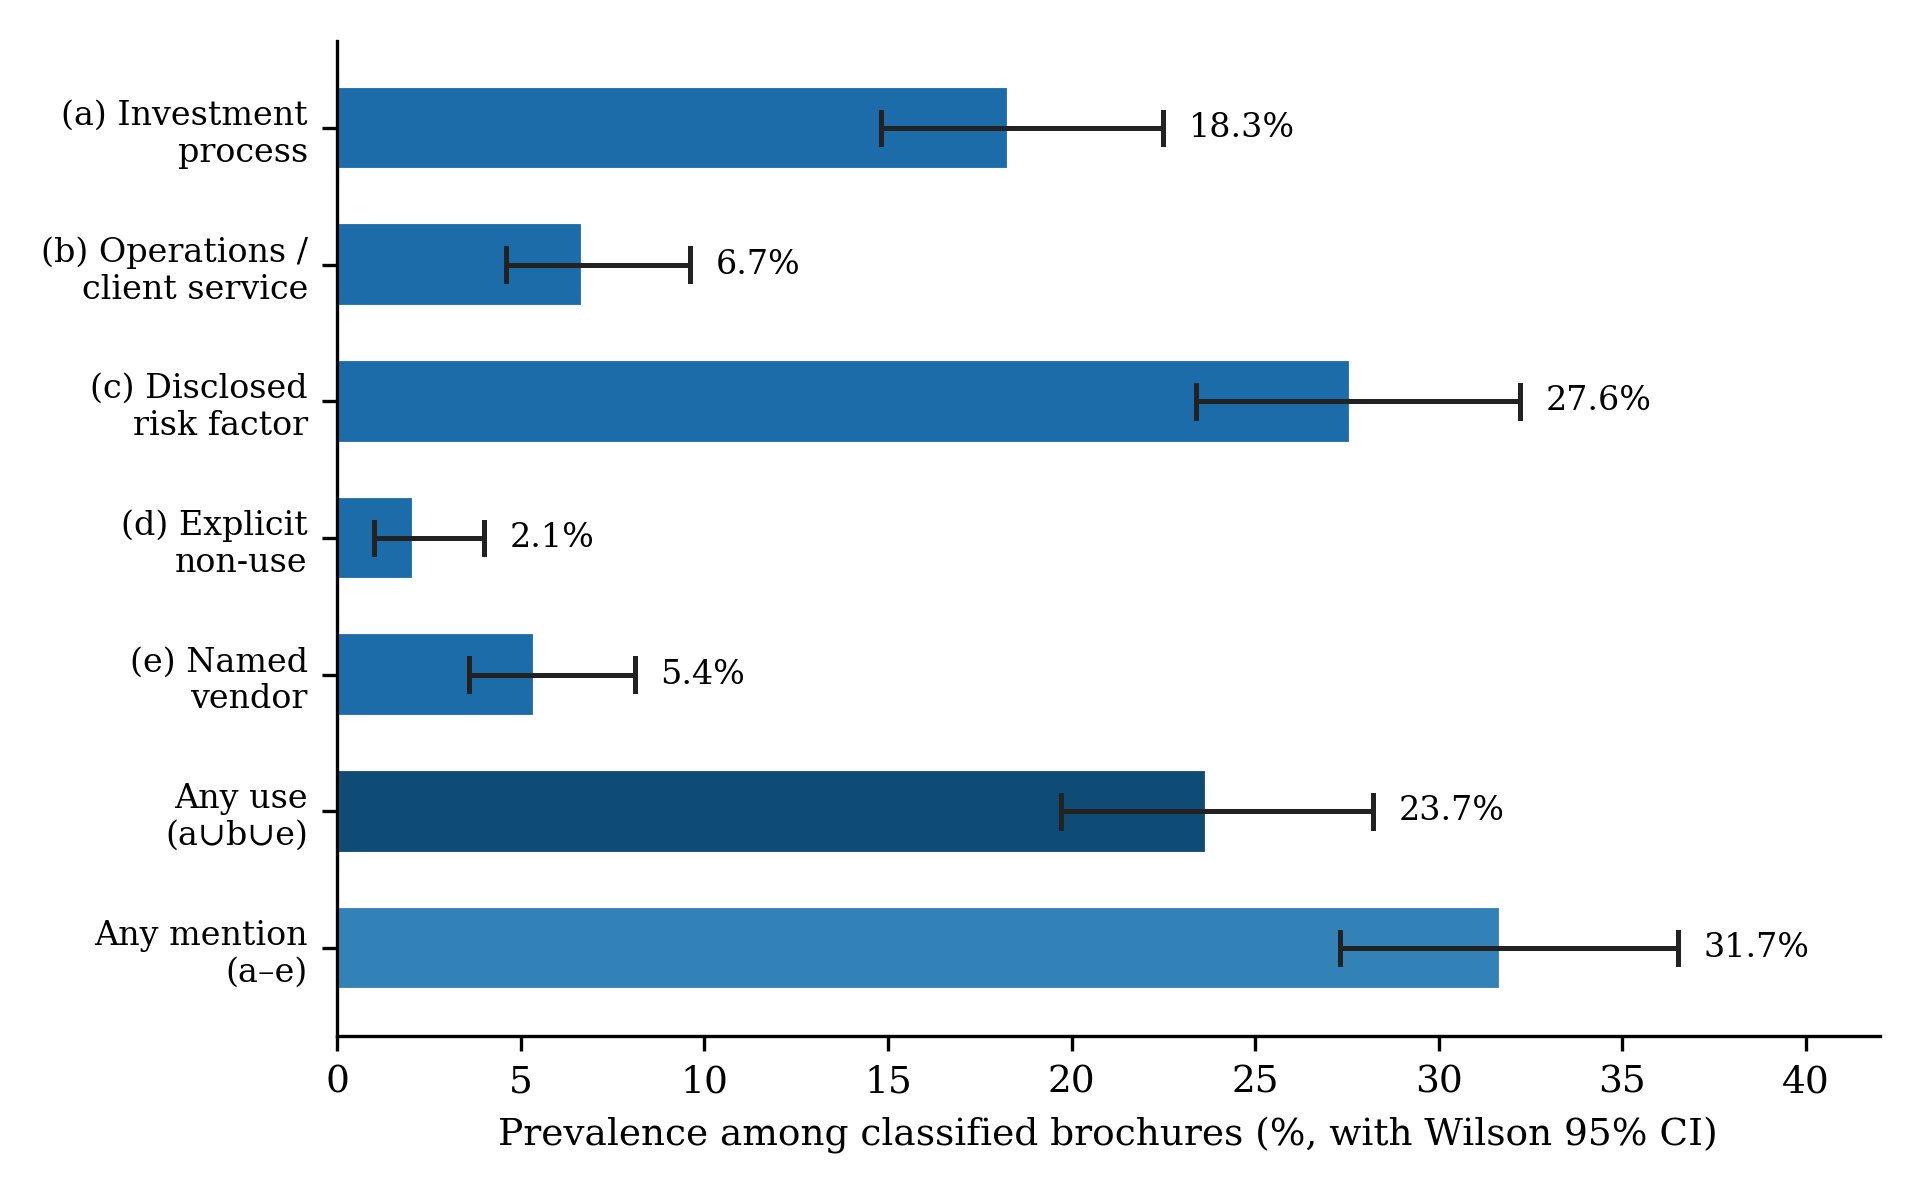
\includegraphics[width=12cm]{figure1_typology}
\end{center}
\caption{Prevalence of each typology label among the 388 classified brochures, with Wilson 95\% confidence intervals. The dominant single label is a risk-factor disclosure (c), not a claim of use; explicit non-use (d) is essentially absent.}
\label{fig:typology}
\end{figure}

\begin{figure}[!ht]
\begin{center}
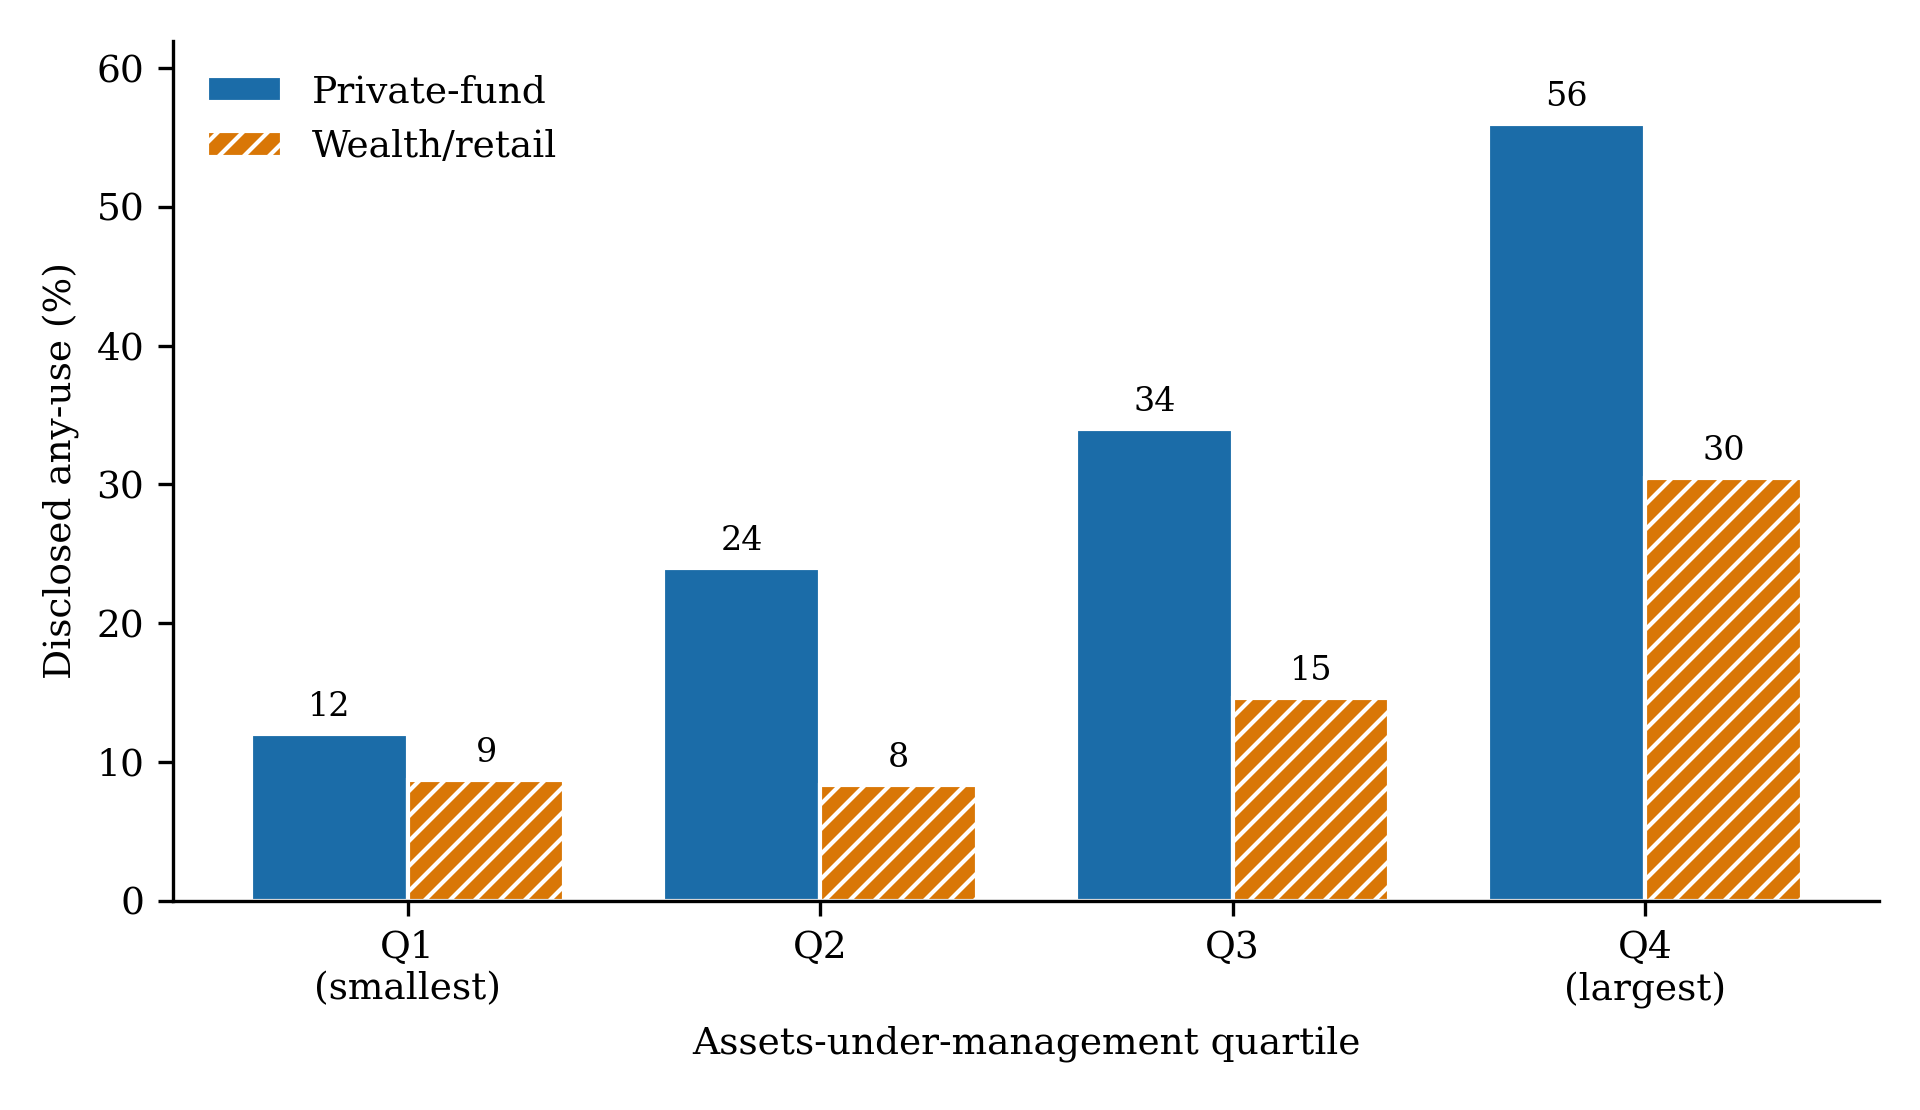
\includegraphics[width=12cm]{figure2_gradient}
\end{center}
\caption{Disclosed any-use of AI by adviser type and AUM quartile. Bars show the within-stratum share of brochures disclosing any use (labels a, b, or e); private-fund advisers (solid) exceed wealth/retail advisers (hatched) at every size quartile, and disclosure rises strongly with size in both types.}
\label{fig:gradient}
\end{figure}

\begin{figure}[!ht]
\begin{center}
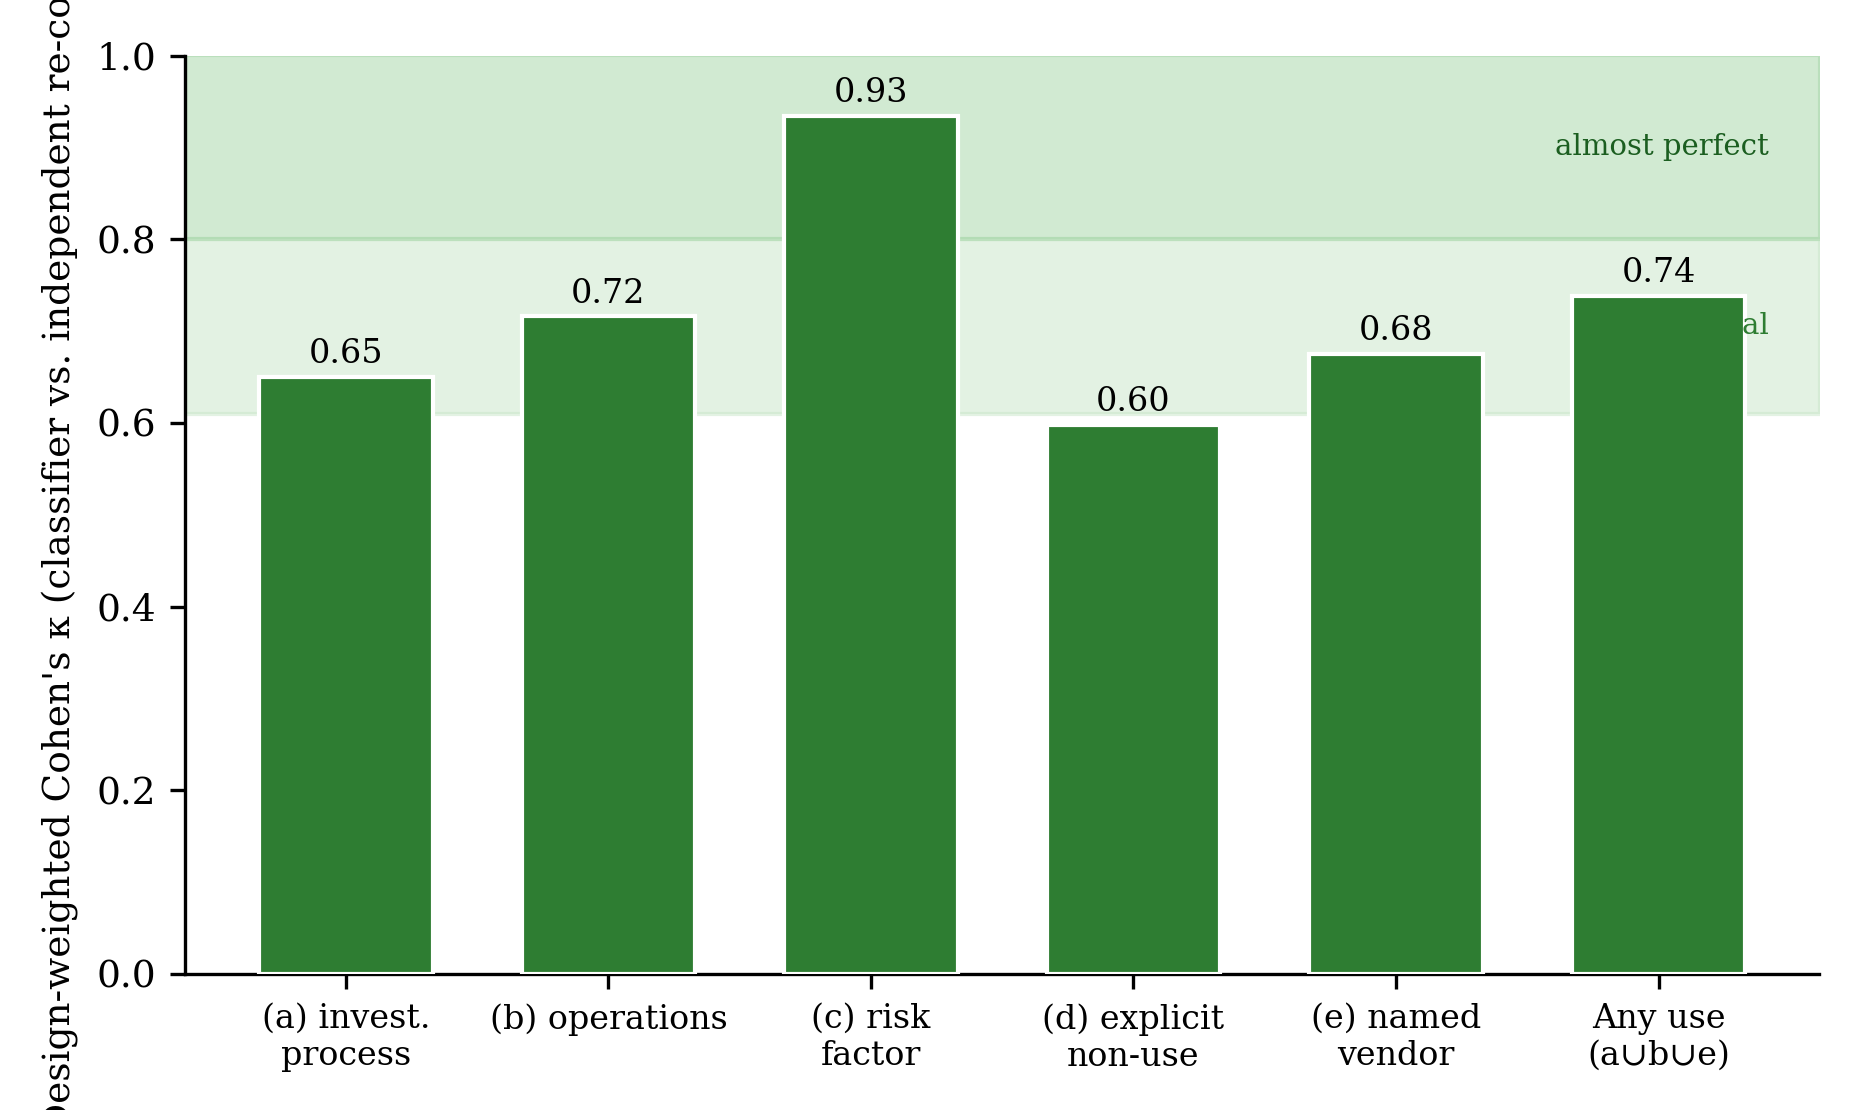
\includegraphics[width=12cm]{figure3_validation}
\end{center}
\caption{Independent cross-family validation: design-weighted Cohen's $\kappa$ between the primary classifier (gpt-4o) and a blinded re-coding by a different model family, per label and for the derived any-use indicator (two-phase verification sample, $n = 180$, weighted to the classified population). Shaded bands mark the conventional substantial (0.61--0.80) and almost-perfect ($>0.80$) agreement regions; the risk-factor label is almost-perfect and any-use is comfortably substantial, while the finer investment-process distinction remains the softest construct.}
\label{fig:validation}
\end{figure}

\begin{figure}[!ht]
\begin{center}
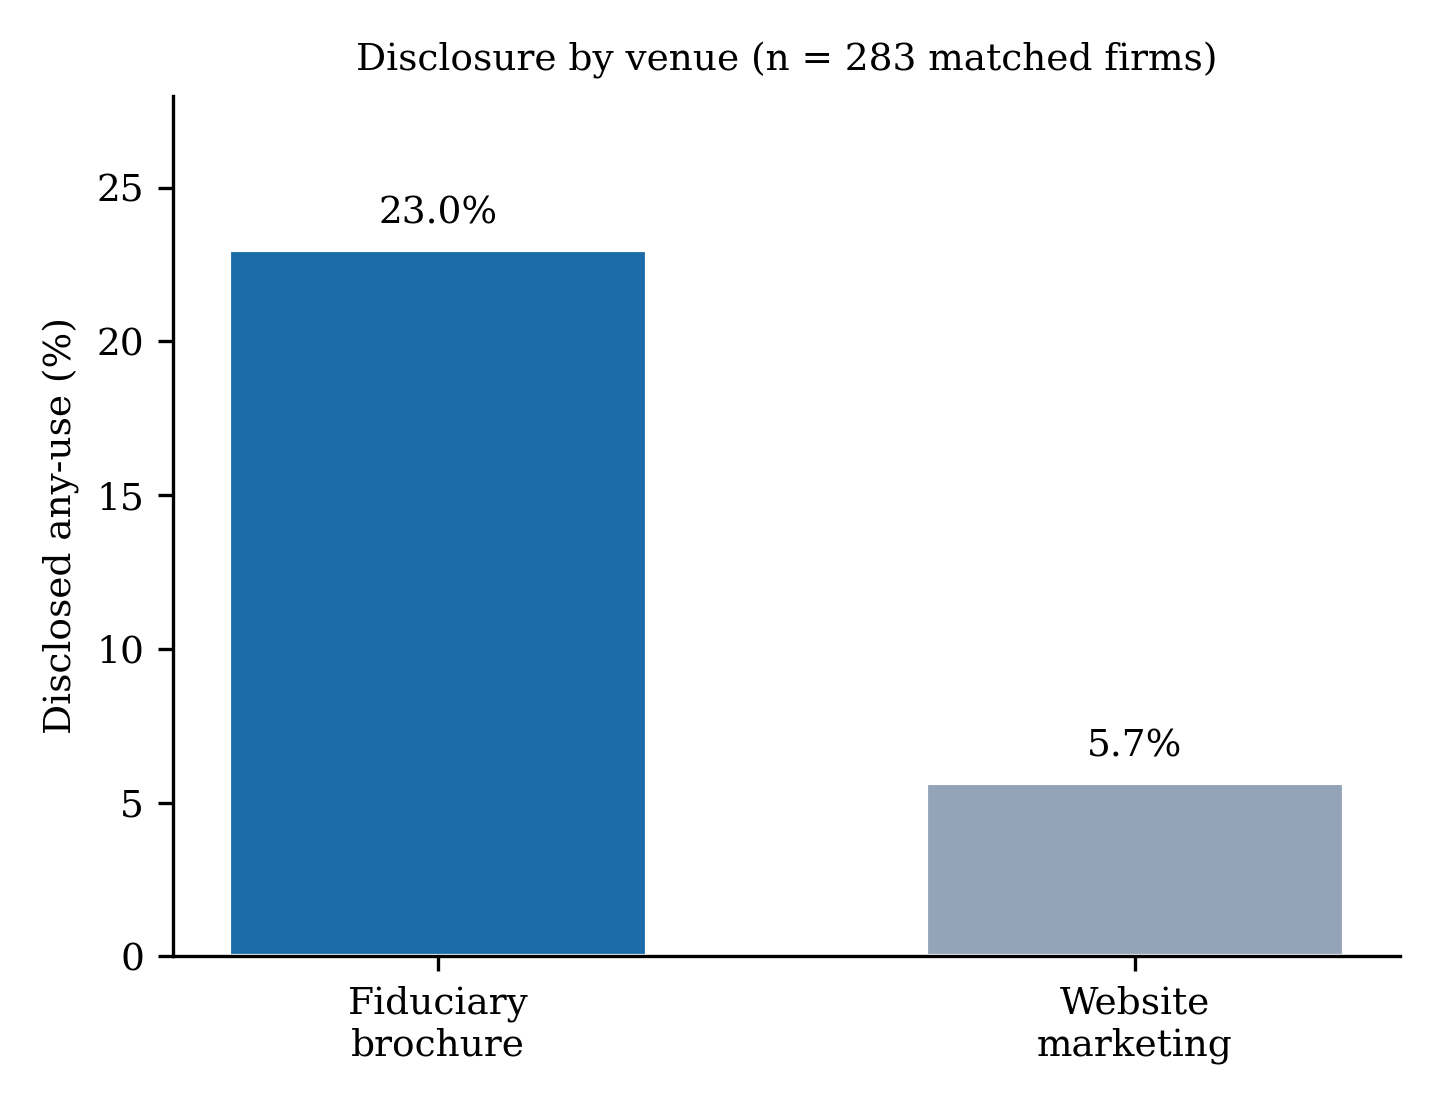
\includegraphics[width=9cm]{figure4_venue}
\end{center}
\caption{Disclosed any-use of AI by venue for the 283 firms observed in both venues. Contrary to the intuition motivating AI-washing concern, the fiduciary brochure is the more AI-forward venue: disclosed use is 23.0\% in brochures versus 5.7\% in current website marketing.}
\label{fig:venue}
\end{figure}

\end{document}
